\documentclass[journal]{IEEEtran}
\usepackage[a5paper, margin=10mm]{geometry}
%\usepackage{lmodern} % Ensure lmodern is loaded for pdflatex
\usepackage{tfrupee} % Include tfrupee package


\setlength{\headheight}{1cm} % Set the height of the header box
\setlength{\headsep}{0mm}     % Set the distance between the header box and the top of the text


%\usepackage[a5paper, top=10mm, bottom=10mm, left=10mm, right=10mm]{geometry}

%
\setlength{\intextsep}{10pt} % Space between text and floats

\makeindex


\usepackage{cite}
\usepackage{amsmath,amssymb,amsfonts,amsthm}
\usepackage{algorithmic}
\usepackage{graphicx}
\usepackage{textcomp}
\usepackage{xcolor}
\usepackage{txfonts}
\usepackage{listings}
\usepackage{enumitem}
\usepackage{mathtools}
\usepackage{gensymb}
\usepackage{comment}
\usepackage[breaklinks=true]{hyperref}
\usepackage{tkz-euclide} 
\usepackage{listings}
\usepackage{multicol}
\usepackage{xparse}
\usepackage{gvv}
%\def\inputGnumericTable{}                                 
\usepackage[latin1]{inputenc}                                
\usepackage{color}                                            
\usepackage{array}                                            
\usepackage{longtable}                                       
\usepackage{calc}                                             
\usepackage{multirow}                                         
\usepackage{hhline}                                           
\usepackage{ifthen}                                               
\usepackage{lscape}
\usepackage{tabularx}
\usepackage{array}
\usepackage{float}
\usepackage{ar}
\usepackage[version=4]{mhchem}


\newtheorem{theorem}{Theorem}[section]
\newtheorem{problem}{Problem}
\newtheorem{proposition}{Proposition}[section]
\newtheorem{lemma}{Lemma}[section]
\newtheorem{corollary}[theorem]{Corollary}
\newtheorem{example}{Example}[section]
\newtheorem{definition}[problem]{Definition}
\newcommand{\BEQA}{\begin{eqnarray}}
\newcommand{\EEQA}{\end{eqnarray}}

\theoremstyle{remark}


\begin{document}
\bibliographystyle{IEEEtran}
\onecolumn

\title{12.873}
\author{INDHIRESH S- EE25BTECH11027}
\maketitle


\renewcommand{\thefigure}{\theenumi}
\renewcommand{\thetable}{\theenumi}

\textbf{Question}.Consider a Cartesian coordinate system defined over a 3-dimensional vector space with orthogonal unit basis vectors $\hat{i}$
$\hat{j}$ and $\Hat{k}$. Let vector $\Vec{a}=\sqrt{2}\hat{i}+\frac{1}{\sqrt{2}}\hat{j}+\hat{k}$ and
vector $\Vec{b}=\frac{1}{\sqrt{2}}\hat{i}+\sqrt{2}\hat{j}-\hat{k}$. The inner product of these vectors $(\Vec{a}.\Vec{b})$ is\\
\textbf{Solution}:
The given vectors can be given as:
\begin{align}
 \Vec{a}=\myvec{\sqrt{2}\\\frac{1}{\sqrt{2}}\\1}\\
 \Vec{b}=\myvec{\frac{1}{\sqrt{2}}\\\sqrt{2}\\-1}
\end{align}
And also
\begin{align}
\Vec{a}.\Vec{b}=\Vec{a}^T\Vec{b}
\end{align}
\begin{align}
 \Vec{a}^T\Vec{b}=\myvec{\sqrt{2}\\\frac{1}{\sqrt{2}}\\1}^T\myvec{\frac{1}{\sqrt{2}}\\\sqrt{2}\\-1}
\end{align}

\begin{align}
    \Vec{a}^T\Vec{b}=1+1-1
\end{align}

\begin{align}
 \Vec{a}^T\Vec{b}=1
\end{align}
\begin{align}
    \Vec{a}.\Vec{b}=1
\end{align}

\begin{figure}[h]
    \centering
    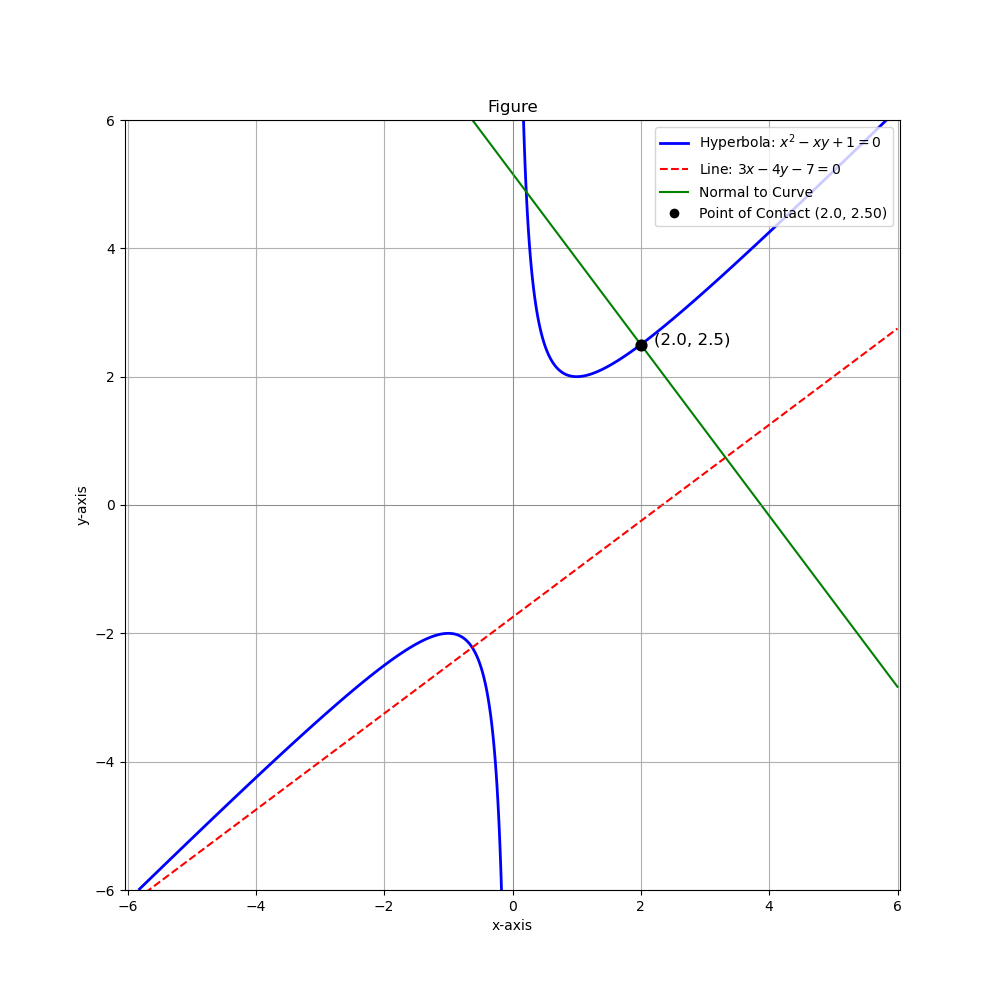
\includegraphics[height=0.5\textheight, keepaspectratio]{figs/figure1.png}
    \label{figure_1}
\end{figure}

\end{document}